% \documentclass{book}

\documentclass[12pt]{article}
\usepackage[pdfborder={0 0 0.5 [3 2]}]{hyperref}%
\usepackage[left=1in,right=1in,top=1in,bottom=1in]{geometry}%
\usepackage[shortalphabetic]{amsrefs}%
\usepackage{amsmath}
\usepackage{enumerate}
\usepackage{enumitem}
\usepackage{amssymb}                
\usepackage{amsmath}                
\usepackage{amsfonts}
\usepackage{amsthm}
\usepackage{bbm}
\usepackage[table,xcdraw]{xcolor}
\usepackage{tikz}
\usepackage{float}
\usepackage{booktabs}
\usepackage{svg}
\usepackage{mathtools}
\usepackage{cool}
\usepackage{url}
\usepackage{graphicx,epsfig}
\usepackage{makecell}
\usepackage{array}

\def\noi{\noindent}
\def\T{{\mathbb T}}
\def\R{{\mathbb R}}
\def\N{{\mathbb N}}
\def\C{{\mathbb C}}
\def\Z{{\mathbb Z}}
\def\P{{\mathbb P}}
\def\E{{\mathbb E}}
\def\Q{\mathbb{Q}}
\def\ind{{\mathbb I}}

\graphicspath{ {images4/} }

\begin{document}
\section*{7 Feb 2017}
We want to verify that the eigenvalues of the integrated operator $E''(u*)$ are what we expect. They should all lie on the real axis since this operator is self-adjoint.\\

\subsection*{Fourier spectral methods}
Since the Fourier differential operators are self-adjoint, we start here. We use domain size $L = 50$, scaled to the interval $[0, 2 \pi]$. Spectrum is found with eig, since matrices aren't too big.
\begin{enumerate}
	\item Single pulse and spectrum
	\begin{figure}[H]
	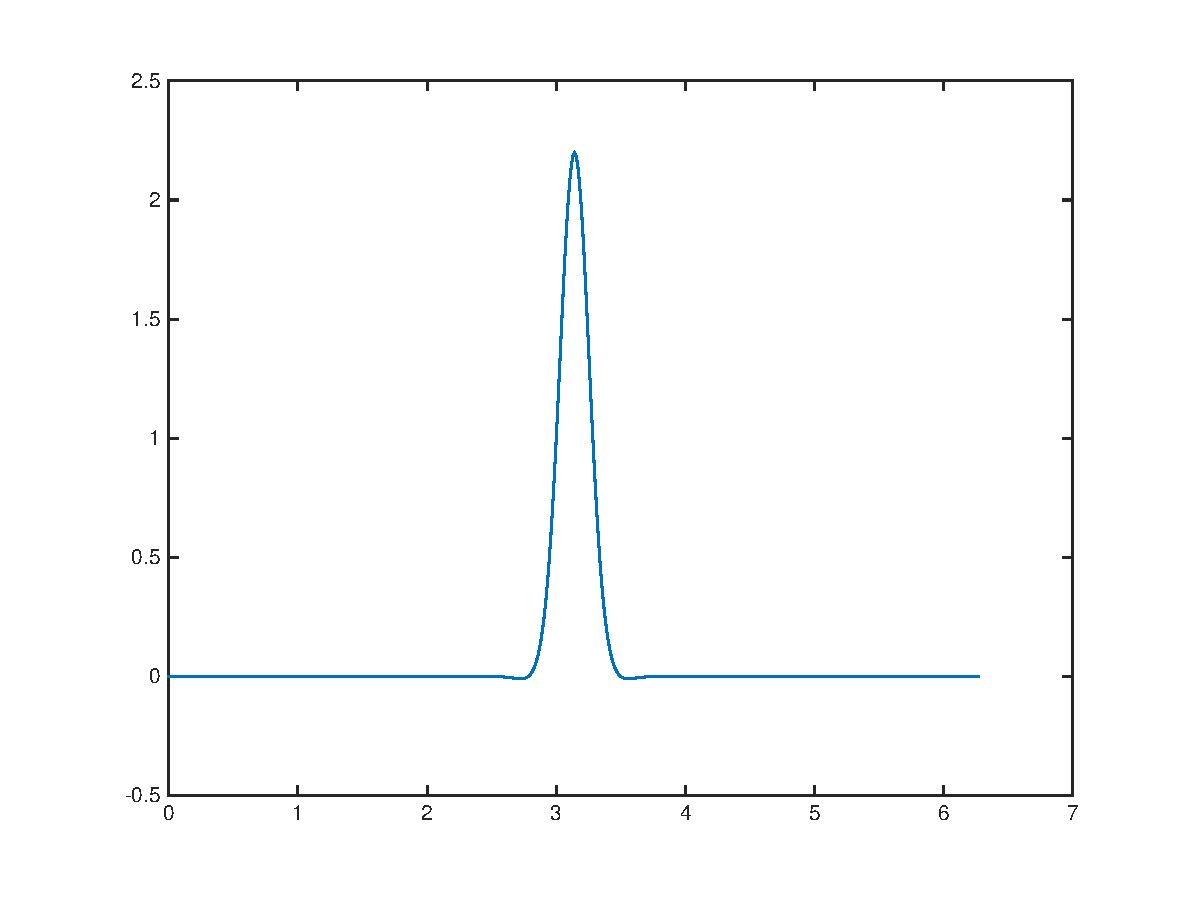
\includegraphics[width=8.5cm]{fouriersinglepulse.eps}
	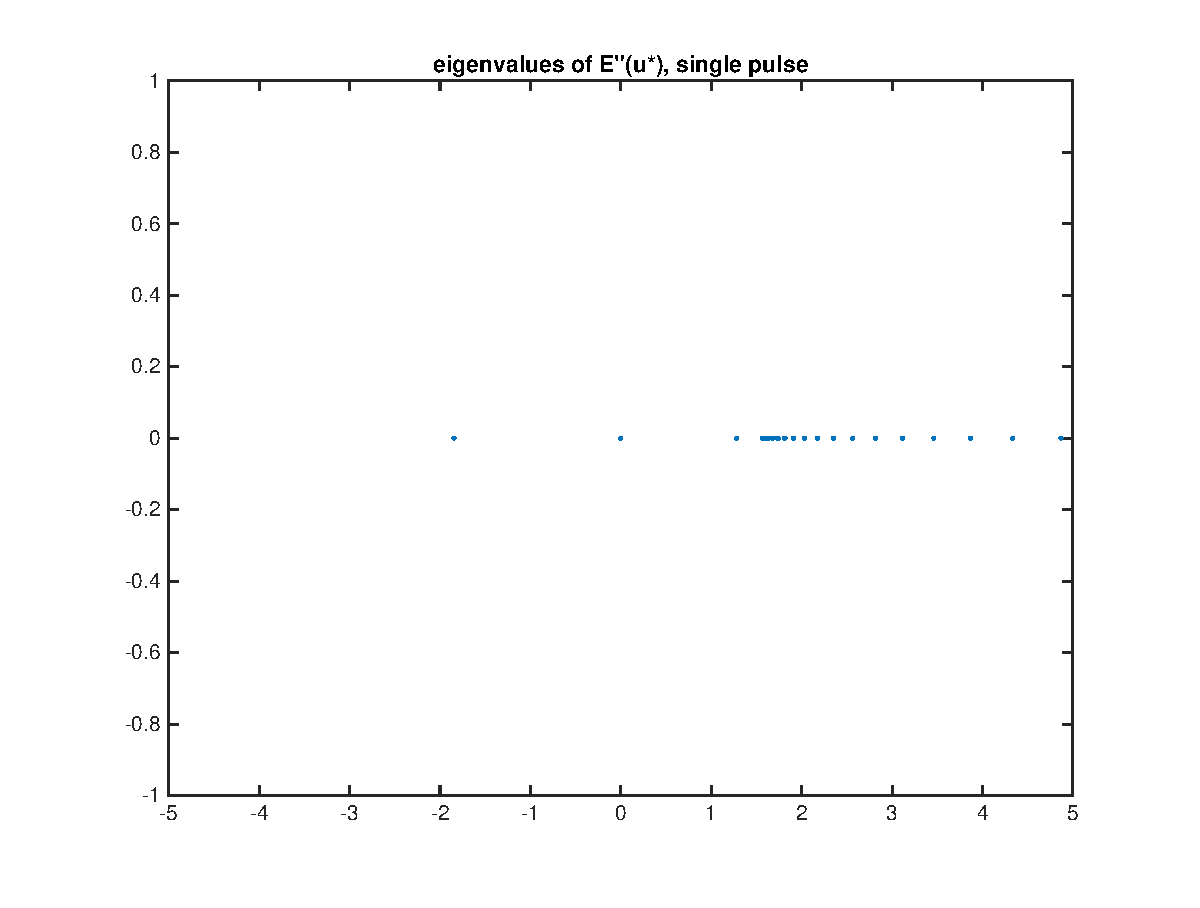
\includegraphics[width=8.5cm]{intEigs1.eps}
	\end{figure}
	This looks exactly as we expect!

	\item Double pulse (joined at first min/max) and spectrum
	\begin{figure}[H]
	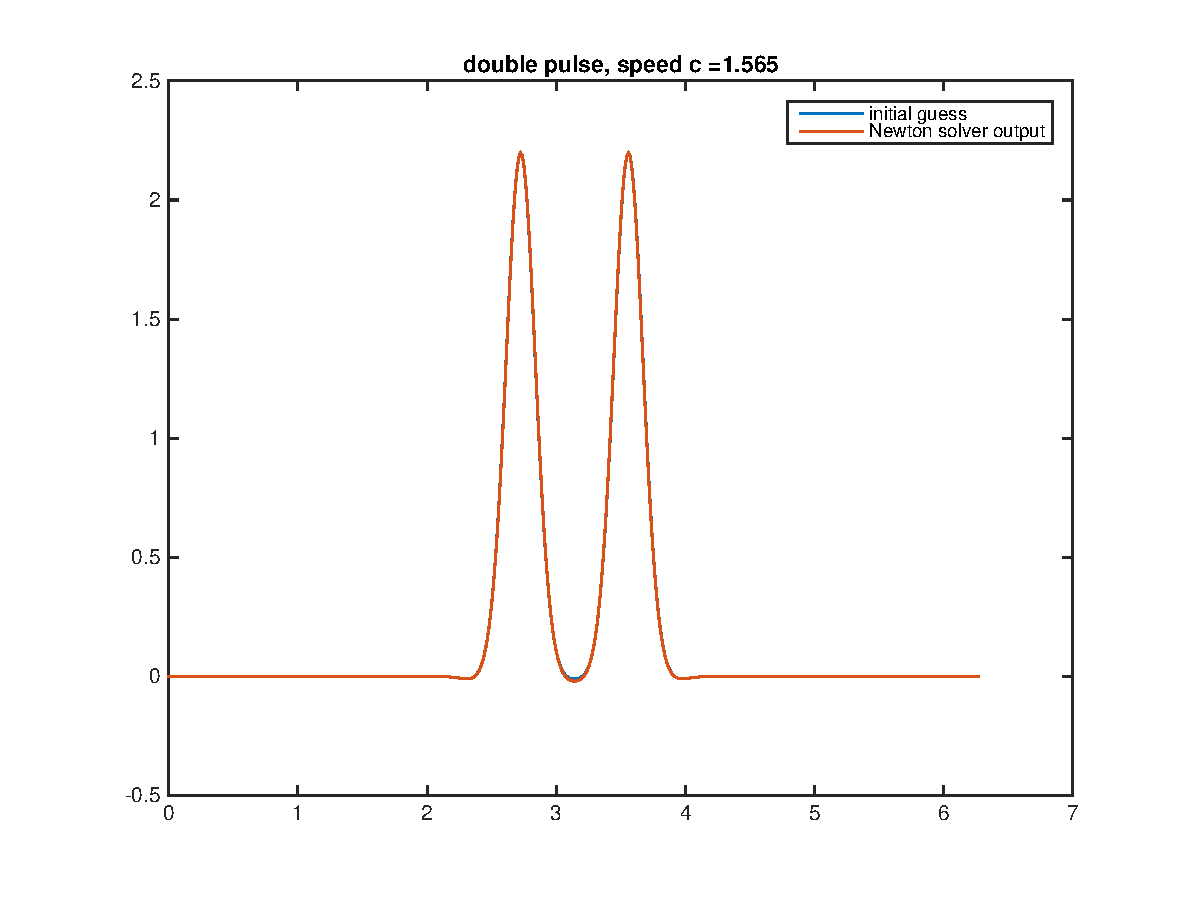
\includegraphics[width=8.5cm]{fourierdoublepulse1.eps}
	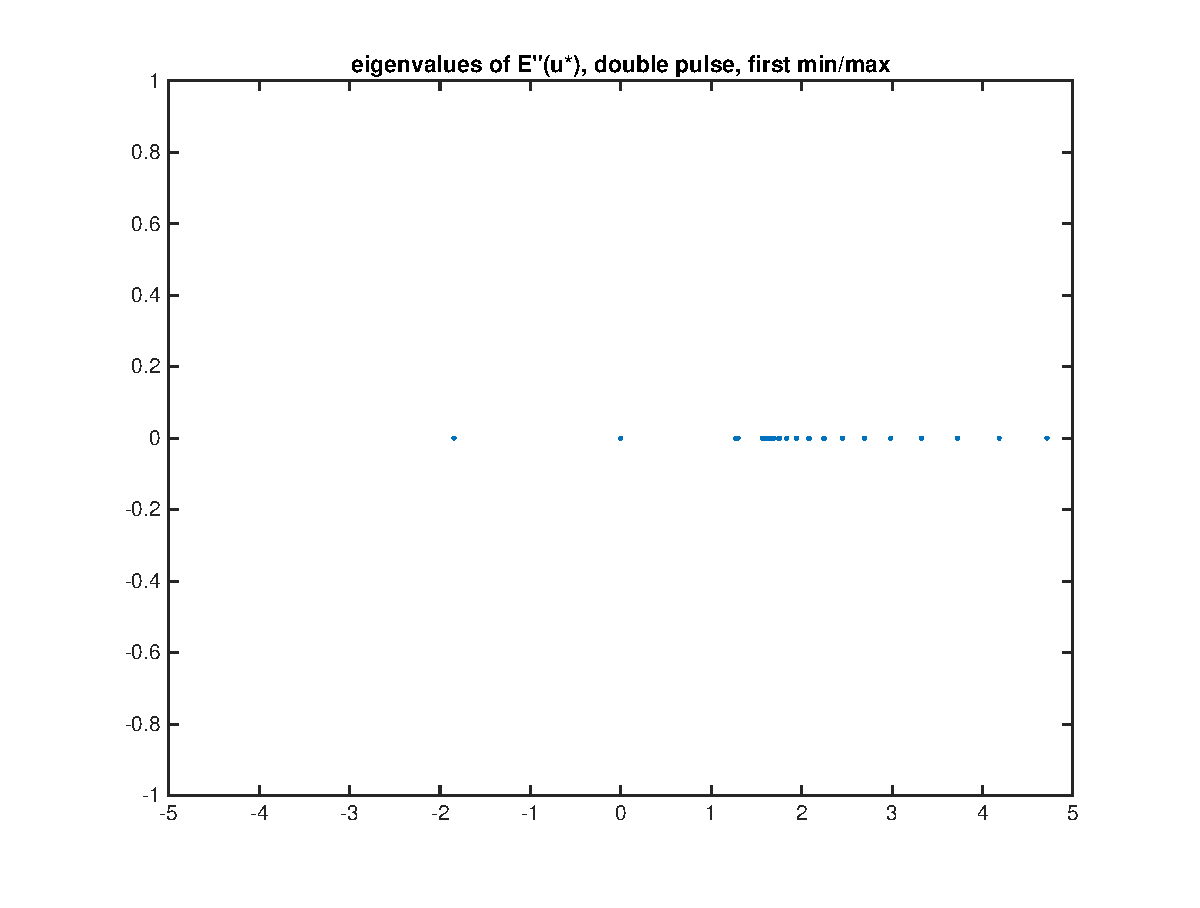
\includegraphics[width=8.5cm]{intEigs2.eps}
	\end{figure}
	If zoom into the leftmost two points, we see that they are both doublets, as expected.
	\begin{figure}[H]
	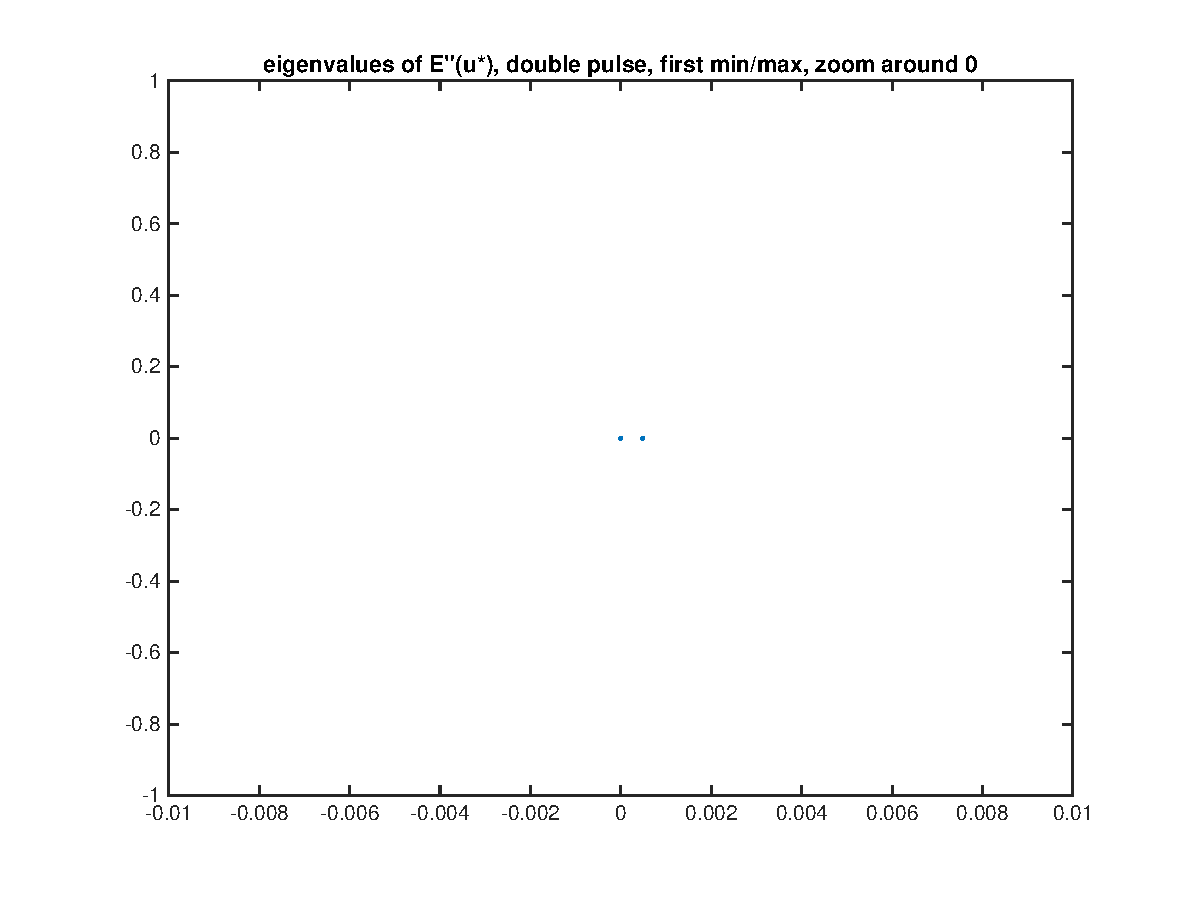
\includegraphics[width=8.5cm]{intEigs2Zoom1.eps}
	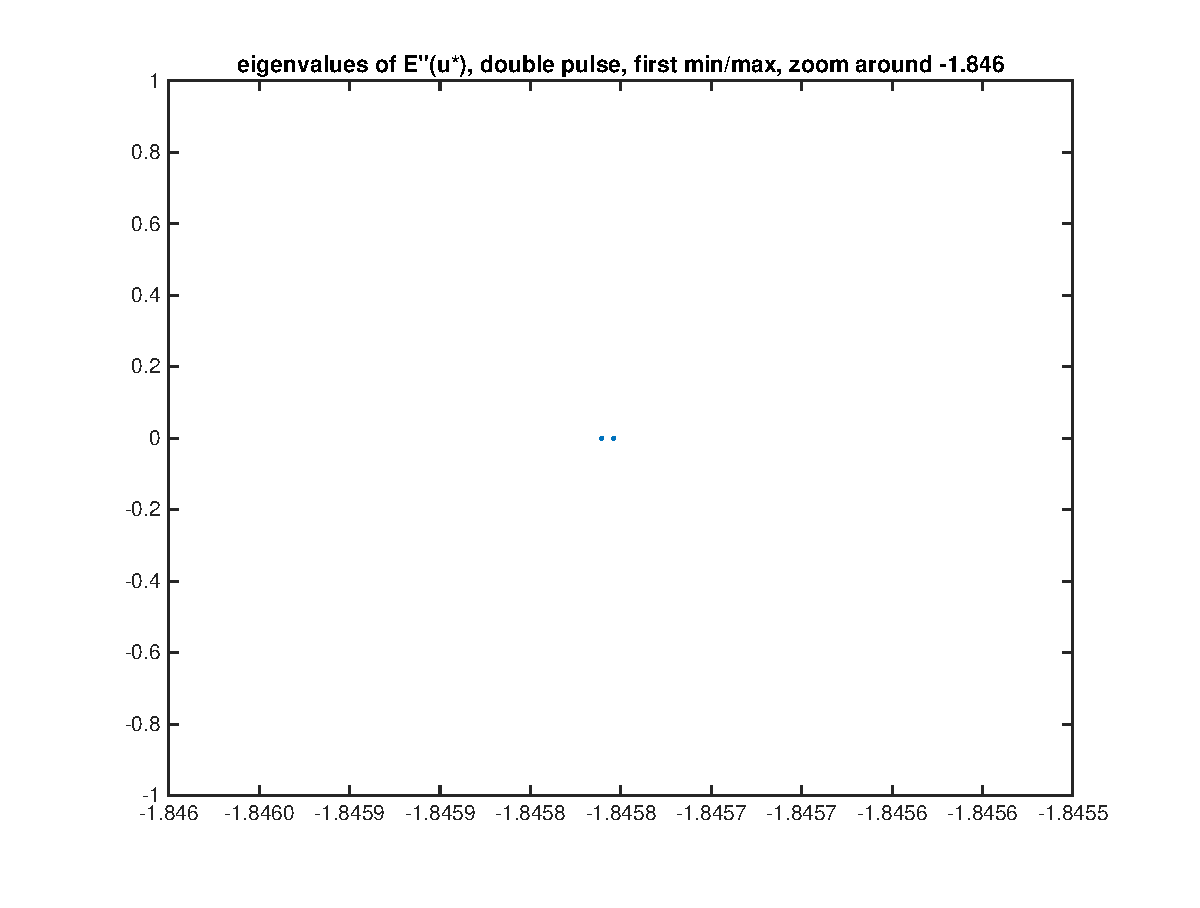
\includegraphics[width=8.5cm]{intEigs2Zoom2.eps}
	\end{figure}
\end{enumerate}

\subsection*{Finite Difference Methods}
Here we use finite difference methods with Neumann boundary conditions. Domain length is $L = 100$, and we have 3999 grid points for the full wave (2000 for the half wave). Here we use eigs to find the spectrum since the matrices are much larger and my computer is slow. The operator here is self-adjoint except for at the boundary, but since we are using Neumann BCs, I think this is ok. In any case, the results are the same as above. Plots of the pulses are not included this time.

\begin{enumerate}
	\item Single pulse and spectrum
	\begin{figure}[H]
	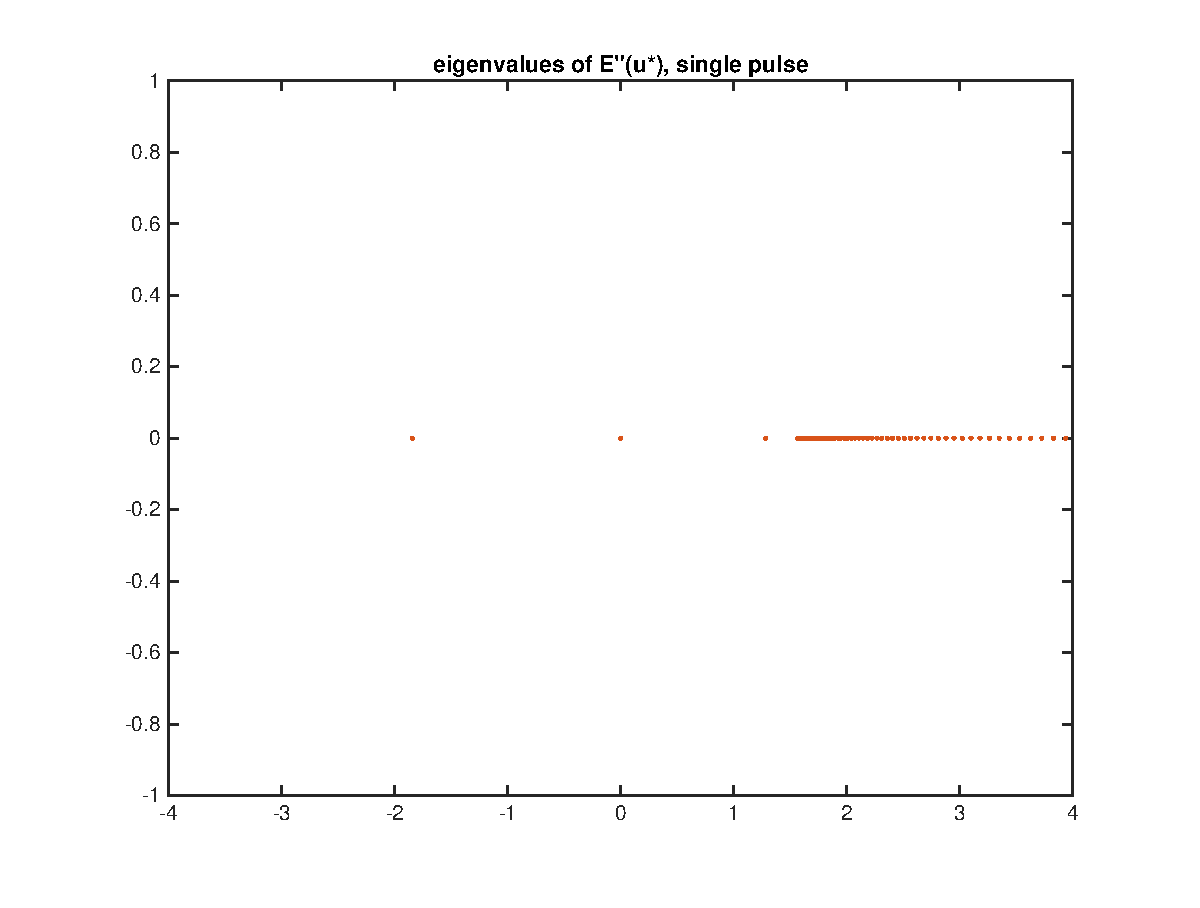
\includegraphics[width=8.5cm]{FDintEigs1.eps}
	\end{figure}

	\item Double pulse (joined at first min/max) and spectrum
	\begin{figure}[H]
	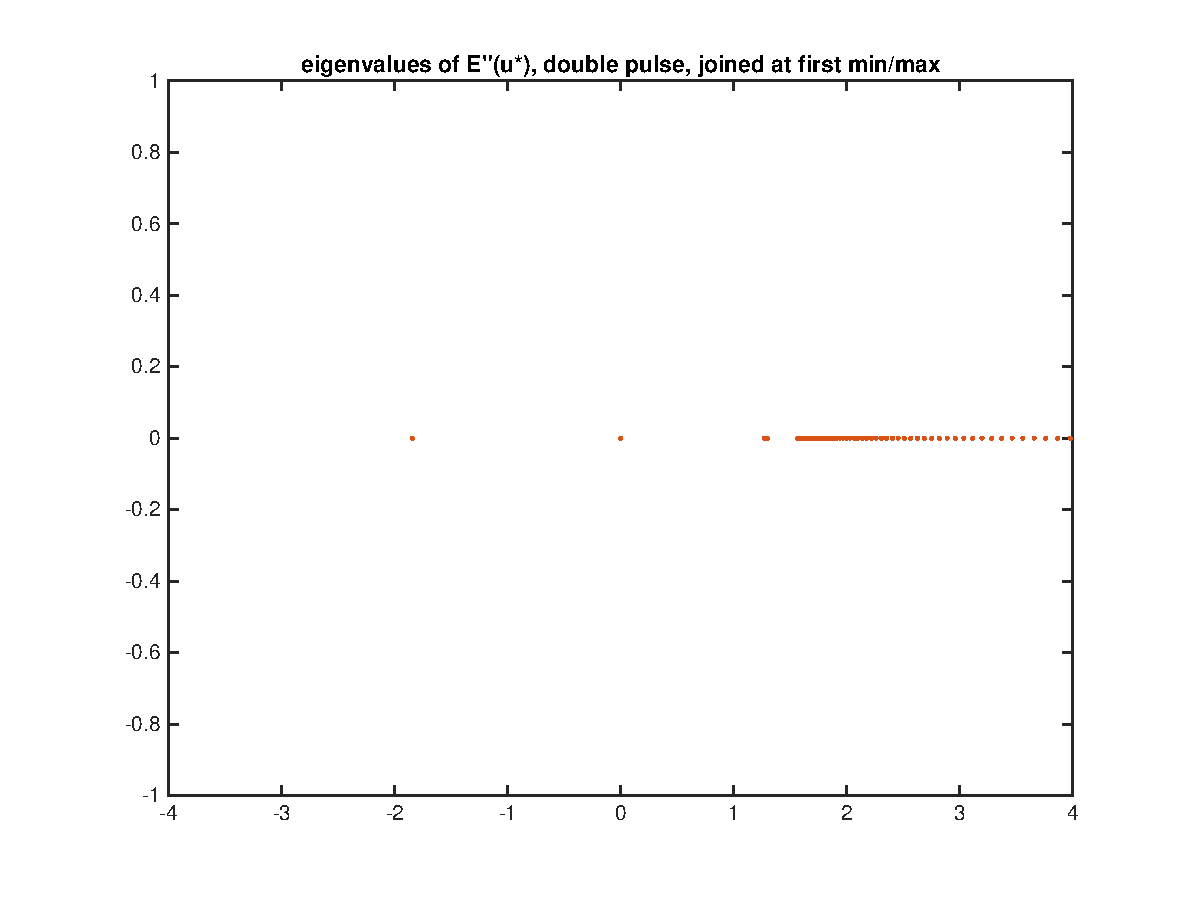
\includegraphics[width=8.5cm]{FDintEigs2.eps}
	\end{figure}
	If zoom into the leftmost two points, we see that they are both doublets, as expected.
	\begin{figure}[H]
	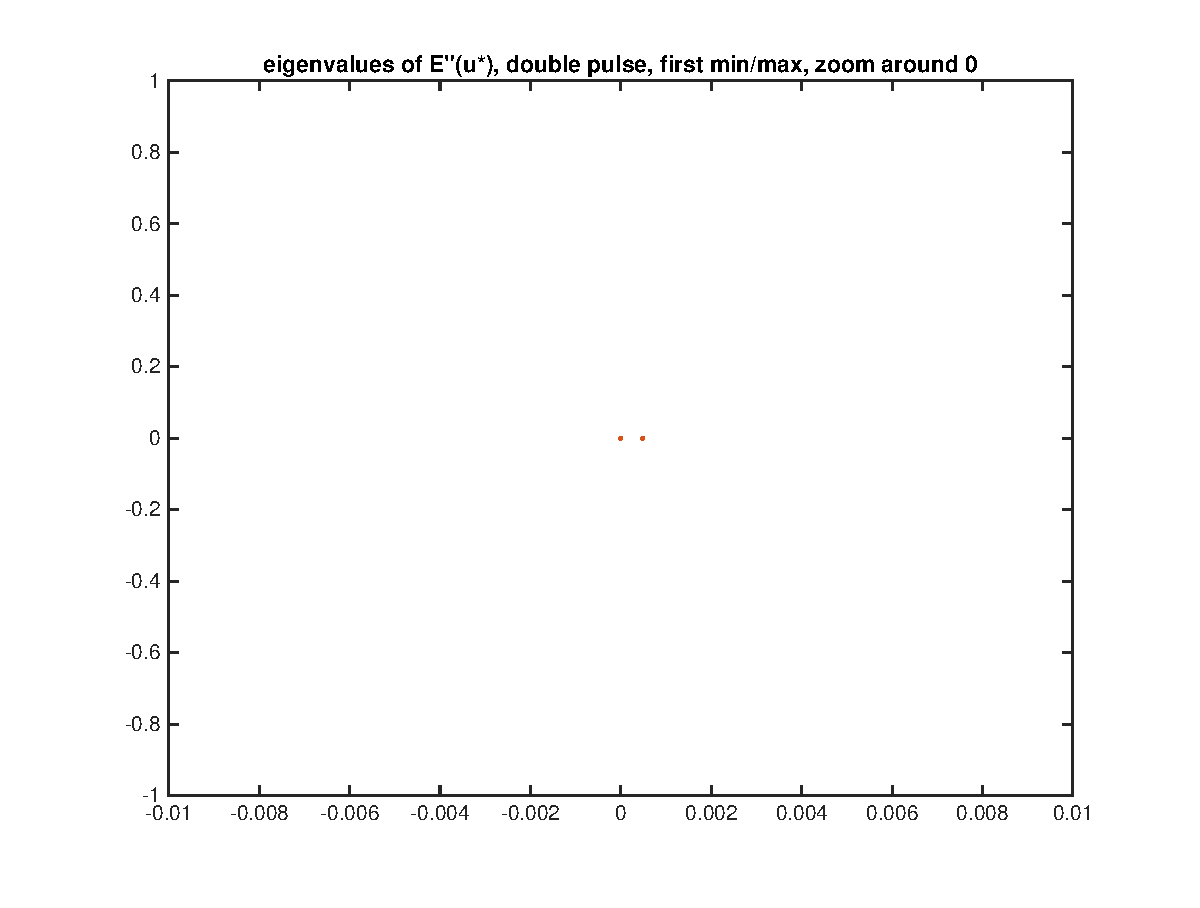
\includegraphics[width=8.5cm]{FDintEigs2Zoom1.eps}
	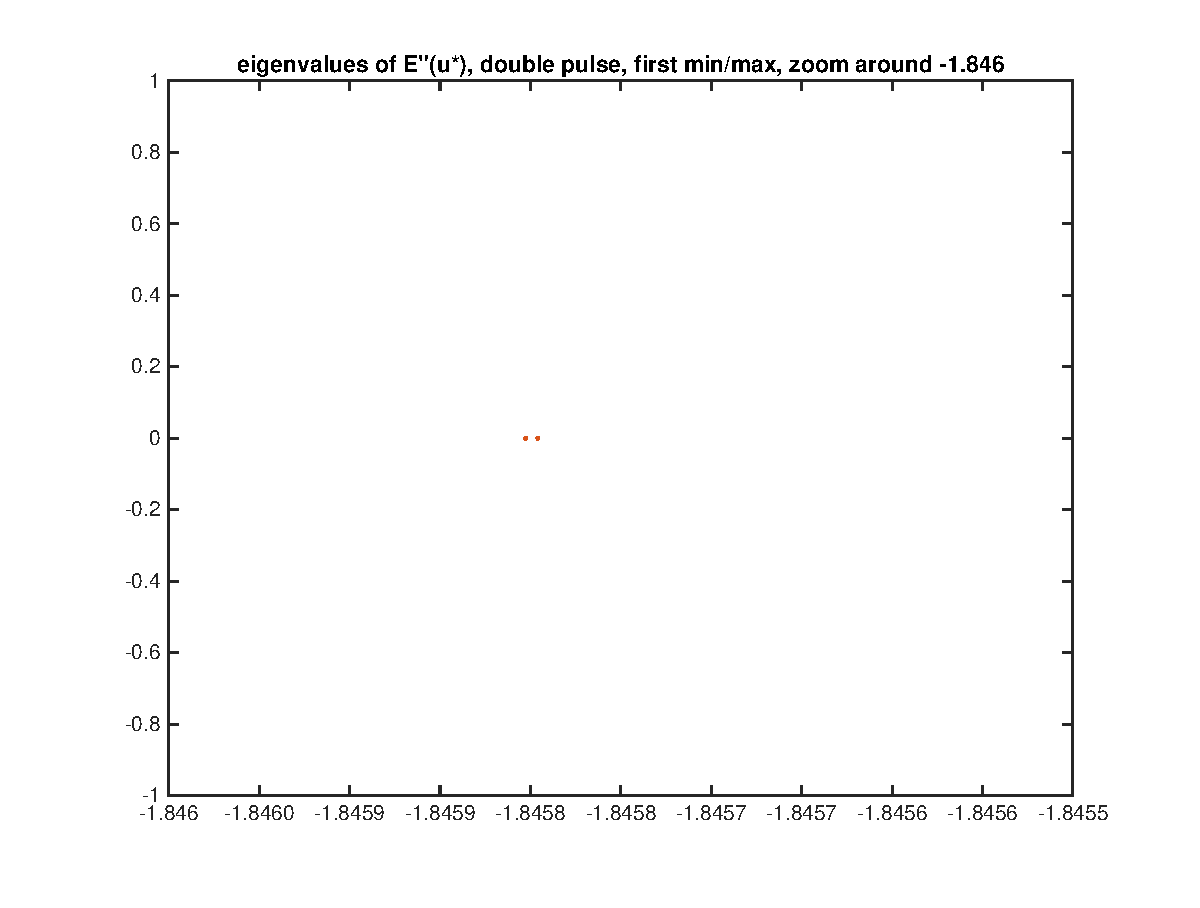
\includegraphics[width=8.5cm]{FDintEigs2Zoom2.eps}
	\end{figure}
\end{enumerate}

\subsection*{Table of eigenvalues}
Here is a table of the eigenvalues near 0 of the integrated operator for the double pulse joined at the first 6 min/max. Finite difference and Fourier spectral methods are compared. In both cases, the domain size is $L = 100$, although it is rescaled to $[0, 2\pi]$ in the Fourier case. For finite differences, 3999 grid points are used. For Fourier spectral methods, 1024 grid points are used.

\begin{figure}[H]
\begin{tabular}{ll|ll|ll}
      &     & Finite Differences &                   & Fourier Spectral  &                   \\
Pulse &     & Eigenvalue near 0  & Paired eigenvalue & Eigenvalue near 0 & Paired eigenvalue \\ \hline
1     & min & -2.2918e-11        & 4.8344e-04        & -2.6904e-10       & 4.8440e-04        \\
2     & max & -1.1339e-11        & 3.2833e-08        & -1.3645e-08       & 2.3140e-08        \\
3     & min & -3.0791e-11        & -3.2869e-11       & 4.1551e-13        & 3.4489e-12        \\
4     & max & -4.5117e-11        & -5.1579e-11       & -4.0409e-14       & 3.6455e-12        \\
5     & min & -4.9293e-11        & -5.1563e-11       & -2.4925e-12       & 3.5353e-12        \\
6     & max & -2.8952e-11        & -3.3429e-11       & 8.3753e-15        & 1.3921e-12       
\end{tabular}
\end{figure}
We expect the paired eigenvalue to ``flip sides'' with every other double pulse, i.e. max on one side, min on the other, but it does not look like that is happening here. For pulses 1 and 2, both FD and Fourier puts the paired eigenvalue on the right. So not sure what is happening. For pulses 3-6, the eigenvalues are so small that we could be running into limitations of the numerical method. Also, the two methods are relatively close for the pulses 1-2, but are much less so for pulses 3-6. Different boundary conditions might explain this, although we are still quite far from the boundary with $L = 100$.

Repeat Fourier spectral methdos with 4096 grid points. The hope was that this would allow eigenvalues to be better distinguished. Unfortunately, this does not appear to be the case. We could conceivably try more grid points, but my computer is too slow to effectively do this.

\begin{figure}[H]
\begin{tabular}{ll|ll}
      &     & Fourier Spectral  & (4096 grid points) \\
Pulse &     & Eigenvalue near 0 & Paired eigenvalue  \\ \hline
1     & min & 3.4148e-11        & 4.8440e-04         \\
2     & max & 2.0651e-10        & 3.7969e-08         \\
3     & min & 3.9457e-11        & 4.5633e-10         \\
4     & max & 1.1101e-11        & 2.0348e-10         \\
5     & min & -5.6576e-12       & -2.6272e-10        \\
6     & max & 7.0752e-11        & 3.1588e-10        
\end{tabular}
\end{figure}

\end{document}

